\lstinputlisting[language=bash,basicstyle=\small]{python_codes/fieldstone_75/keywords.ascii}

\begin{center}
Code at \url{https://github.com/cedrict/fieldstone/tree/master/python_codes/fieldstone_75}
\end{center}

\par\noindent\rule{\textwidth}{0.4pt}

%%%%%%%%%%%%%%%%%%%%%%%%%%%%%%%%%%%%%%%%%%%%%%%%%%%%%%%%%%%%%%%%%%%%%%%%%%%%%%%%%%%%%%%%%%%%

As explained in Section~\ref{ss:quadmini3D}, we could extend the bubbles 
of Lamichhane (2017) \cite{lami17} to 3D in order to enrich the $Q_1$ space:

\begin{eqnarray}
b^{(1)} (r,s,t) &=& (1-r)(1-s)(1-t) \cdot (1-r^2) (1-s^2) (1-t^2) \\
b^{(2)} (r,s,t) &=& (1 + \beta(r+s+t)) \cdot (1-r^2) (1-s^2) (1-t^2) 
\end{eqnarray}

In what follows I set $\beta=1/4$ as I have shown in the 2D case that it does not really matter. 

%..................................................................................
\paragraph{The 'Burstedde' benchmark} It is called like this in the ASPECT manual 
but it originates in Dohrmann \& Bochev (2004) \cite{dobo04}. It is carried 
out with $Q_2 \times Q_1$ elements in Stone 17. 
Relevant python file on github is {\tt stone\_burstedde.py}.

The polynomial solution to the 3D Stokes equation are postulated:
\begin{equation}
\vec{\upnu}
=
\left(
\begin{array}{c}
x+x^2+xy+x^3y \\
y + xy + y^2 + x^2 y^2\\
-2z - 3xz - 3yz - 5x^2 yz
\end{array}
\right)
\end{equation}
and
\begin{equation}
p = xyz + x^3 y^3z - 5/32
\end{equation}
The body force is obtained by inserting the expressions above in the Stokes equations
(see Section~\ref{mms3}) and the viscosity is set to 1.


\begin{center}
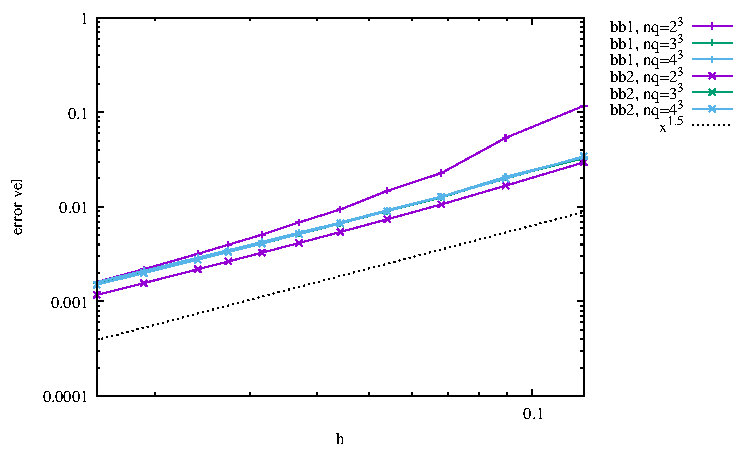
\includegraphics[width=7cm]{python_codes/fieldstone_75/results/burst/errors_v.pdf}
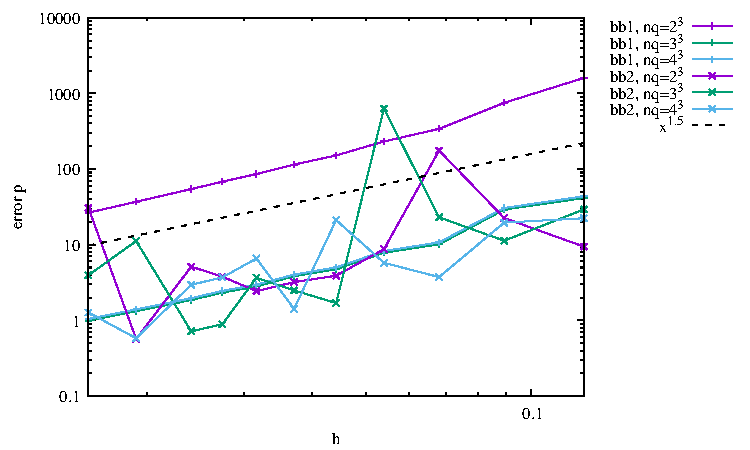
\includegraphics[width=7cm]{python_codes/fieldstone_75/results/burst/errors_p.pdf}\\
{\captionfont $\uparrow$ Velocity and pressure error convergence for both bubbles and with varying number of 
quadrature points nq.}
\end{center}


\begin{center}
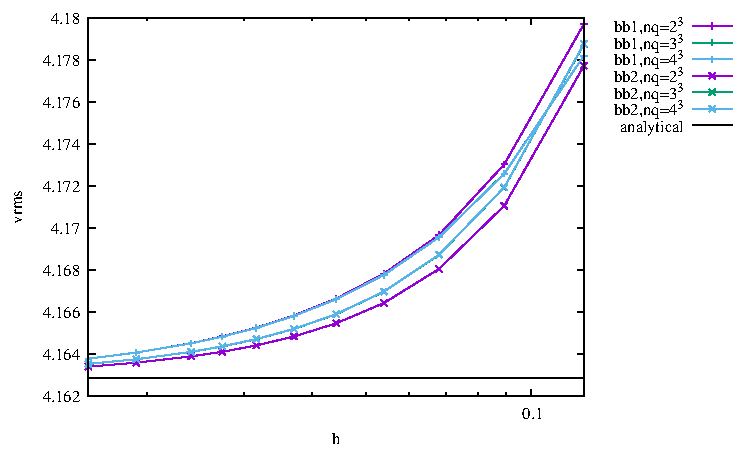
\includegraphics[width=8cm]{python_codes/fieldstone_75/results/burst/vrms.pdf}\\
{\captionfont $\uparrow$ Root mean square velocity for both bubbles and with varying number of   
quadrature points nq.}
\end{center}


\begin{center}
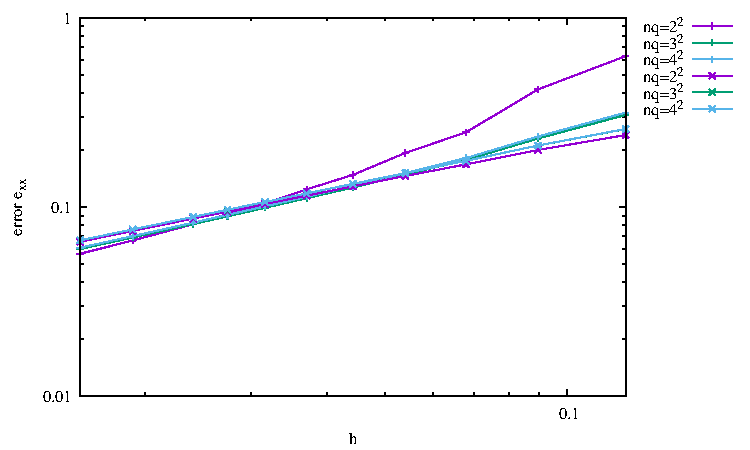
\includegraphics[width=5cm]{python_codes/fieldstone_75/results/burst/errors_exx}
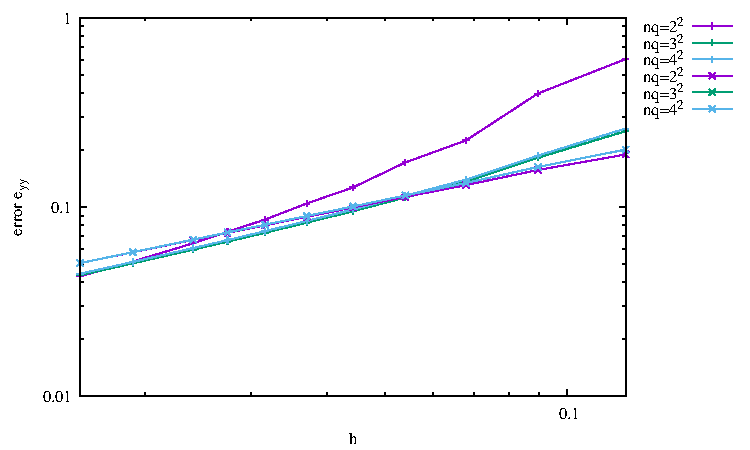
\includegraphics[width=5cm]{python_codes/fieldstone_75/results/burst/errors_eyy}
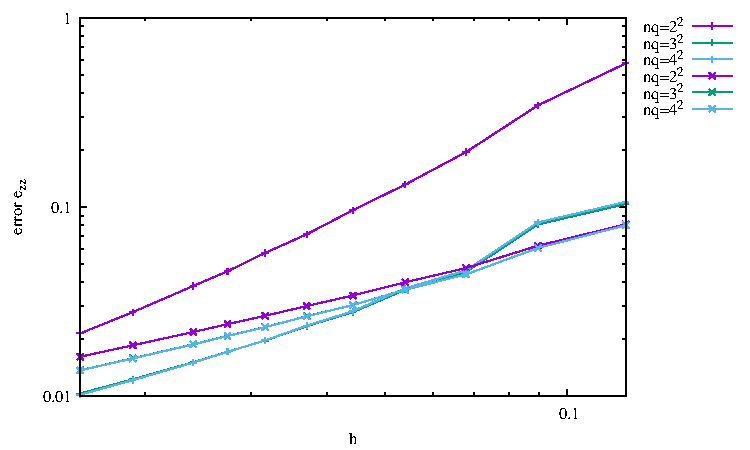
\includegraphics[width=5cm]{python_codes/fieldstone_75/results/burst/errors_ezz}\\
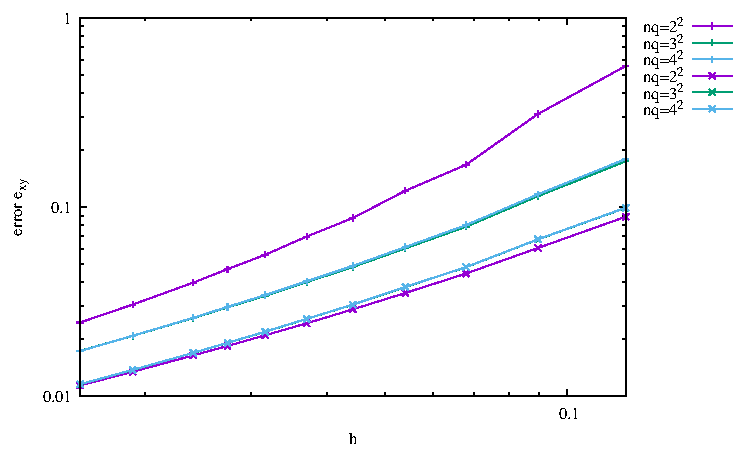
\includegraphics[width=5cm]{python_codes/fieldstone_75/results/burst/errors_exy}
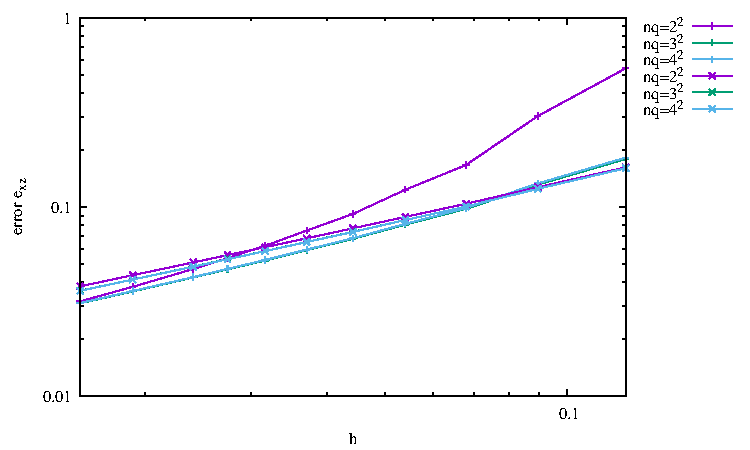
\includegraphics[width=5cm]{python_codes/fieldstone_75/results/burst/errors_exz}
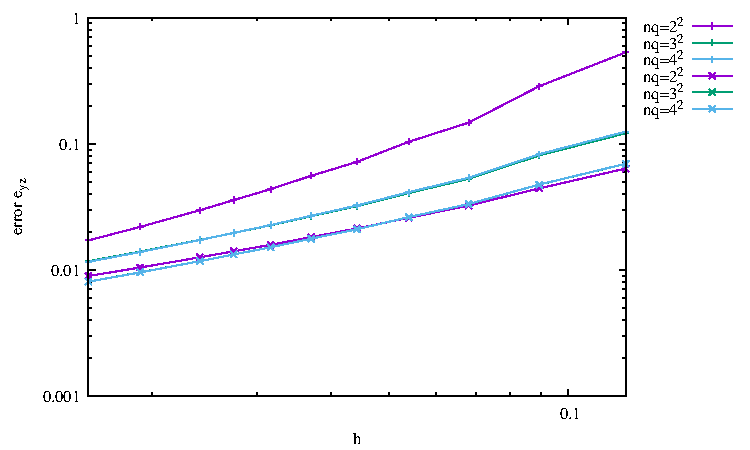
\includegraphics[width=5cm]{python_codes/fieldstone_75/results/burst/errors_eyz}\\
{\captionfont $\uparrow$ Error convergence for the 6 components of the strain rate tensor.}
\end{center}


\begin{center}
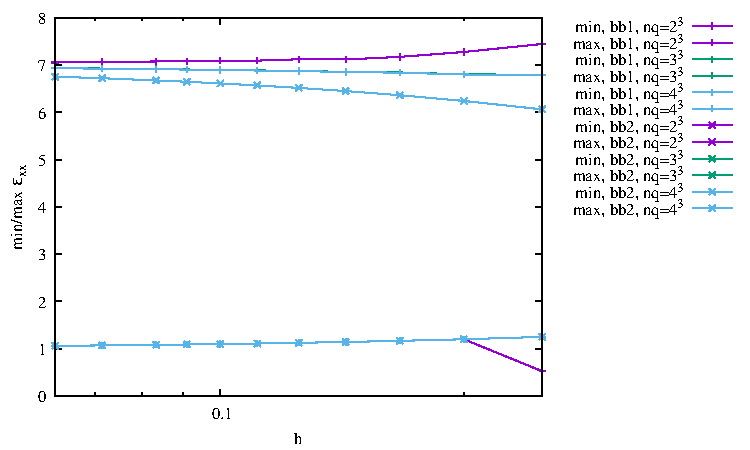
\includegraphics[width=5cm]{python_codes/fieldstone_75/results/burst/exx_stats.pdf}
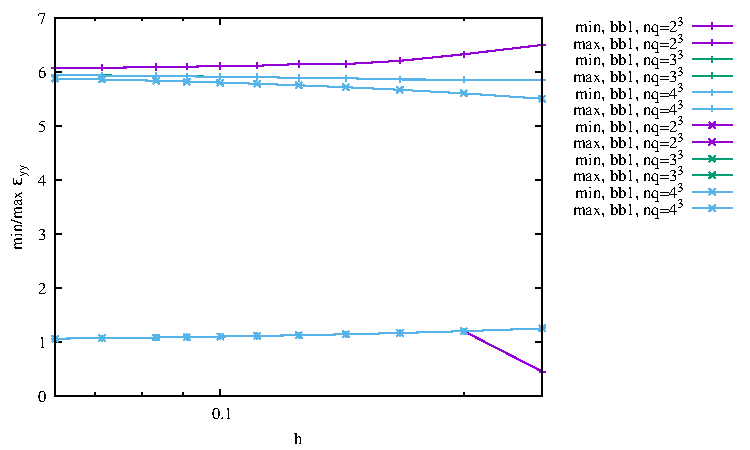
\includegraphics[width=5cm]{python_codes/fieldstone_75/results/burst/eyy_stats.pdf}
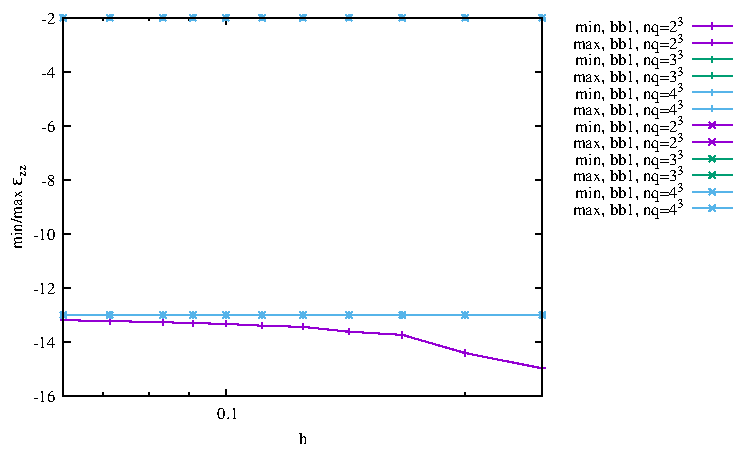
\includegraphics[width=5cm]{python_codes/fieldstone_75/results/burst/ezz_stats.pdf}\\
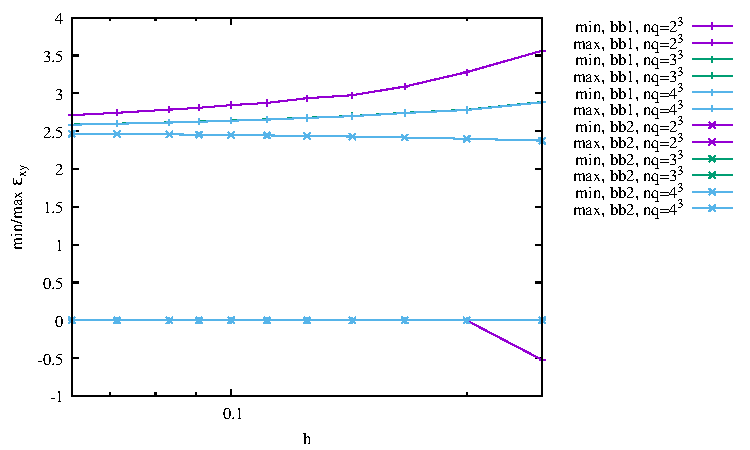
\includegraphics[width=5cm]{python_codes/fieldstone_75/results/burst/exy_stats.pdf}
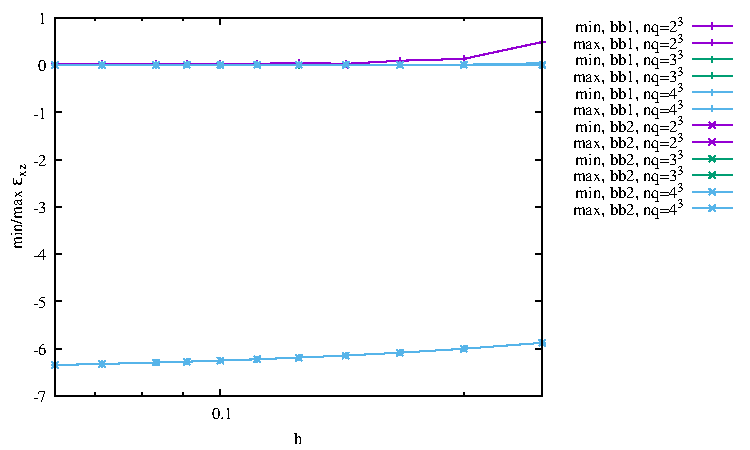
\includegraphics[width=5cm]{python_codes/fieldstone_75/results/burst/exz_stats.pdf}
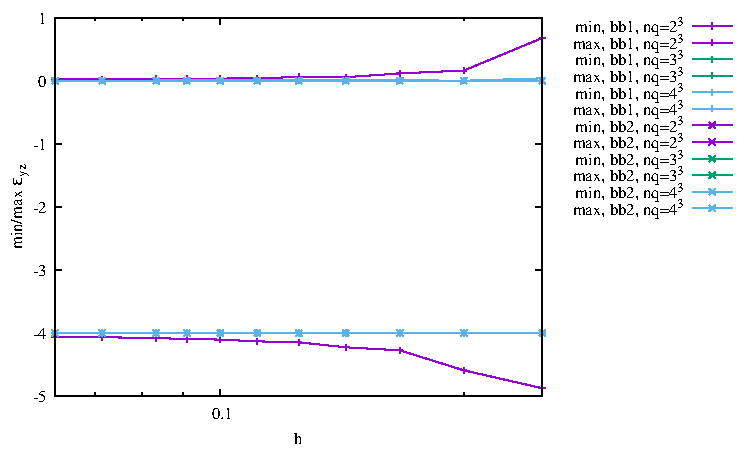
\includegraphics[width=5cm]{python_codes/fieldstone_75/results/burst/eyz_stats.pdf}\\
{\captionfont $\uparrow$ min/max statistics of the 6 components of the strain rate tensor
as a function of the mesh size $h$.}
\end{center}


\begin{center}
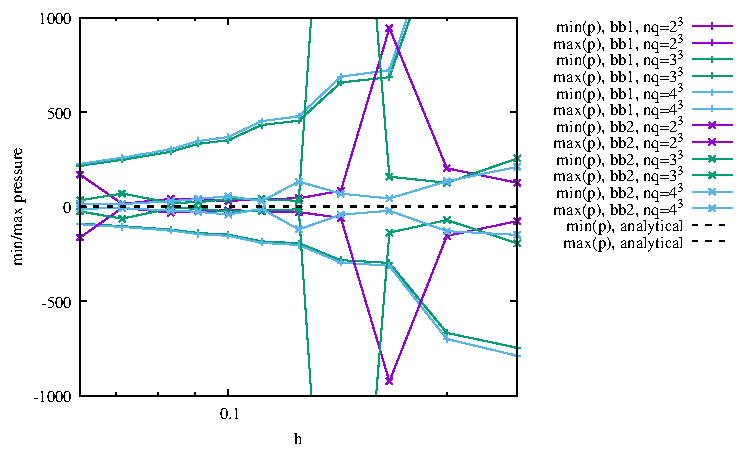
\includegraphics[width=11cm]{python_codes/fieldstone_75/results/burst/p_stats.pdf}\\
{\captionfont $\uparrow$ min/max statistics of the pressure as a function of the mesh size $h$. Note that 
the black dashed lines represent the analytical solution, so that these measurements are some two 
orders of magnitude off.}
\end{center}

\begin{center}
\includegraphics[width=5cm]{python_codes/fieldstone_75/results/burst/vel.png}
\includegraphics[width=5cm]{python_codes/fieldstone_75/results/burst/p_b1}
\includegraphics[width=5cm]{python_codes/fieldstone_75/results/burst/p_b2}\\
{\captionfont From left to right: velocity field; pressure field obtained with bubble 1;
pressure field obtained with bubble 2. Resolution is 12x12x12 elements.}
\end{center}

We see that in this case the bubble \#2 is way worse than bubble \#1. Both 
yield very bad pressure fields, although the pressure min/max value seem to converge 
towards the analytical values for bubble \#1. 
Note that the current code is limited to fairly low resolutions, i.e. about $24^3$ elements so that
I would need to implement a better Stokes solver (e.g. CG on Schur complement) instead 
of building the Stokes system and passing it to the solver as a whole as I do now. %Take it from stone 16. 

It appears that $3^3$ quadrature points always yield better results than $2^3$ points
so I set $nq=3^3$ in what follows.

%...........................................................................
\paragraph{The generic mms3D} In order to verify that 
the above results are robust (or that I have not made a mistake)
I have tried another manufactured solution, as defined in Section~\ref{ss:mms3Dgen}. 
Python file on github is {\tt stone\_mms3D.py}

\begin{eqnarray}
u(x,y,z) &=& x(1-x)(1-2y)(1-2z)\\
v(x,y,z) &=& (1-2x) y(1-y) (1-2z) \\
w(x,y,z) &=& -2(1-2x)(1-2y)z(1-z) \\
p(x,y,z) &=& (2x-1)(2y-1)(2z-1)
\end{eqnarray}

\begin{center}
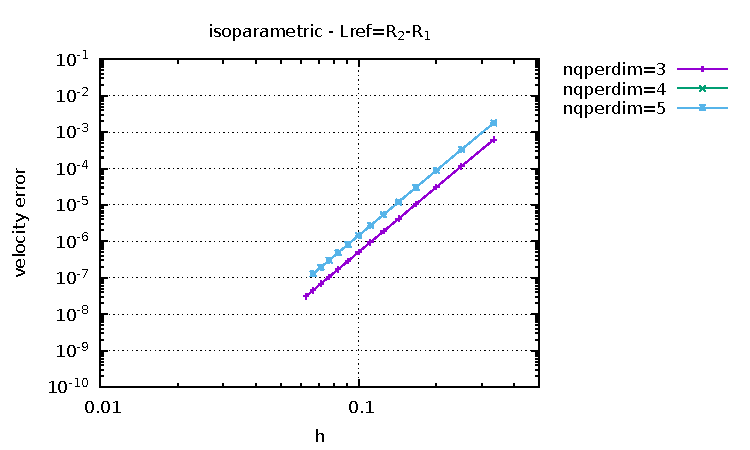
\includegraphics[width=7cm]{python_codes/fieldstone_75/results/mms3D/errors_v.pdf}
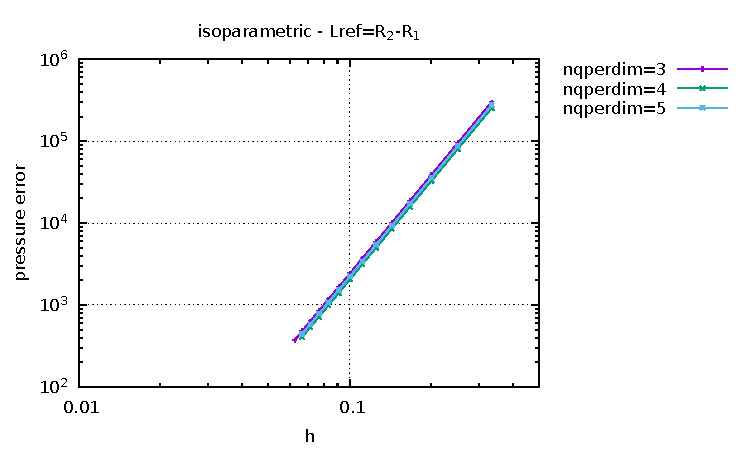
\includegraphics[width=7cm]{python_codes/fieldstone_75/results/mms3D/errors_p.pdf}\\
{\captionfont $\uparrow$ Velocity and pressure error convergence for both bubbles}
\end{center}

\begin{center}
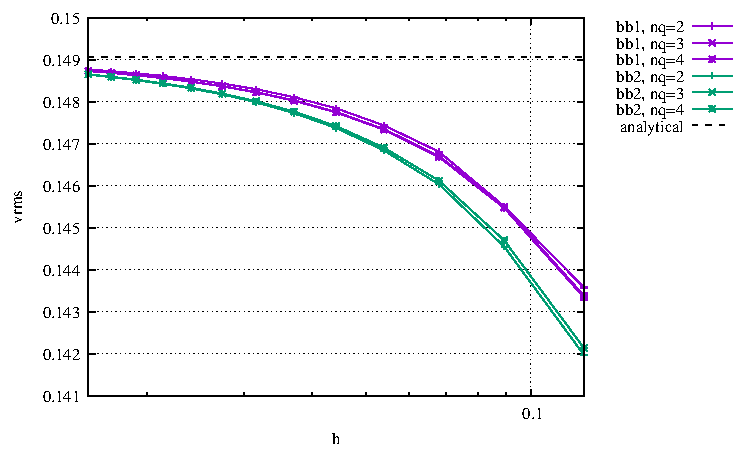
\includegraphics[width=8cm]{python_codes/fieldstone_75/results/mms3D/vrms.pdf}\\
{\captionfont $\uparrow$ Root mean square velocity for both bubbles}
\end{center}

\begin{center}
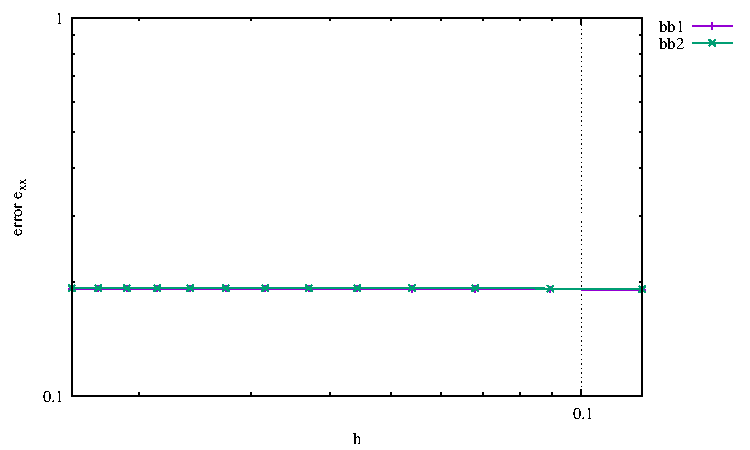
\includegraphics[width=5cm]{python_codes/fieldstone_75/results/mms3D/errors_exx}
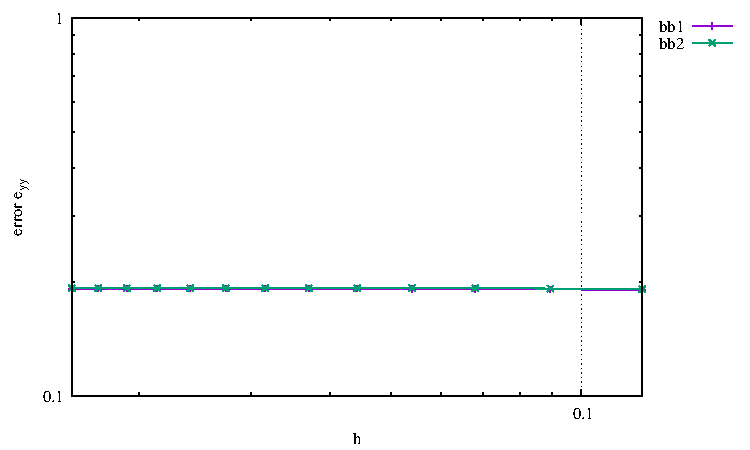
\includegraphics[width=5cm]{python_codes/fieldstone_75/results/mms3D/errors_eyy}
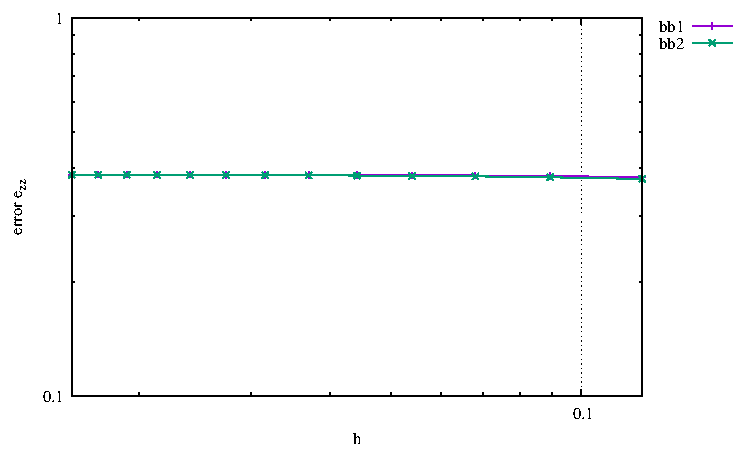
\includegraphics[width=5cm]{python_codes/fieldstone_75/results/mms3D/errors_ezz}\\
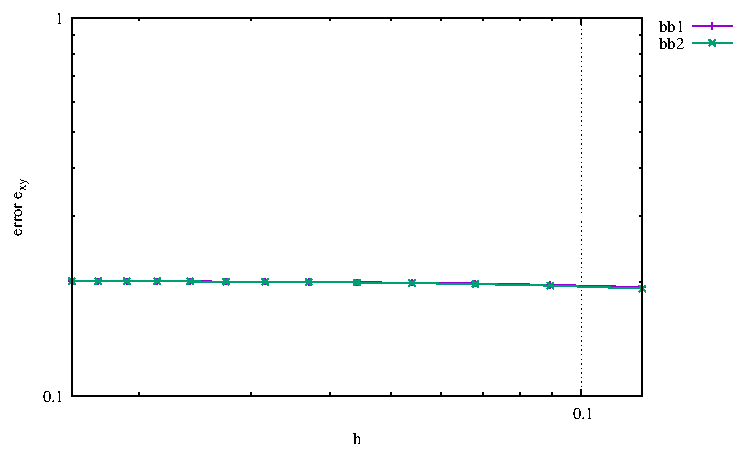
\includegraphics[width=5cm]{python_codes/fieldstone_75/results/mms3D/errors_exy}
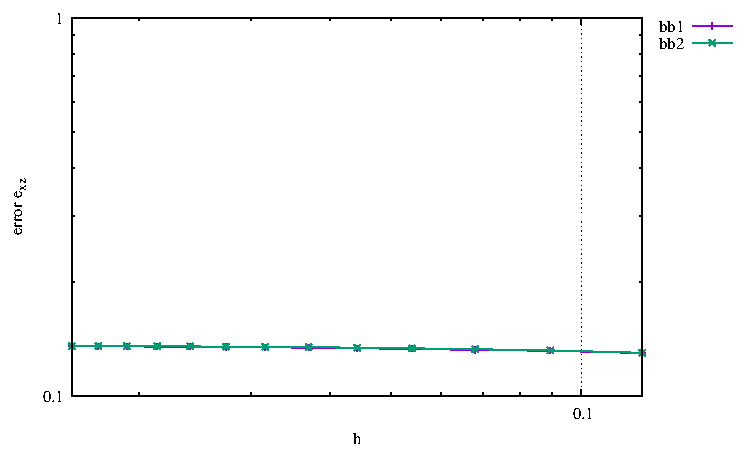
\includegraphics[width=5cm]{python_codes/fieldstone_75/results/mms3D/errors_exz}
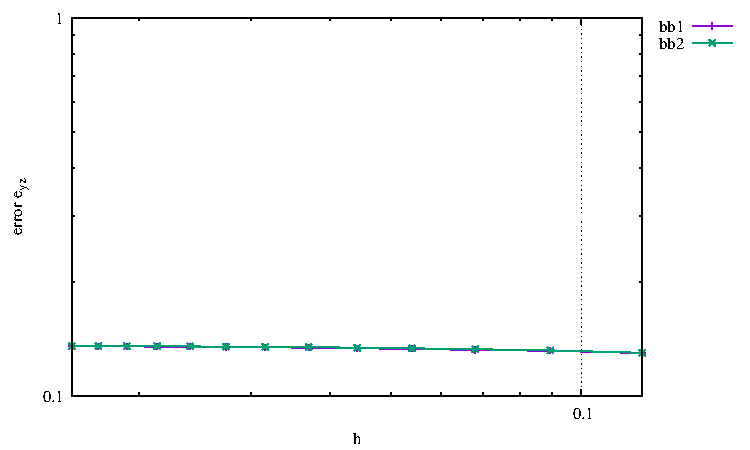
\includegraphics[width=5cm]{python_codes/fieldstone_75/results/mms3D/errors_eyz}\\
{\captionfont $\uparrow$ Error convergence for the 6 components of the strain rate tensor.}
\end{center}

\begin{center}
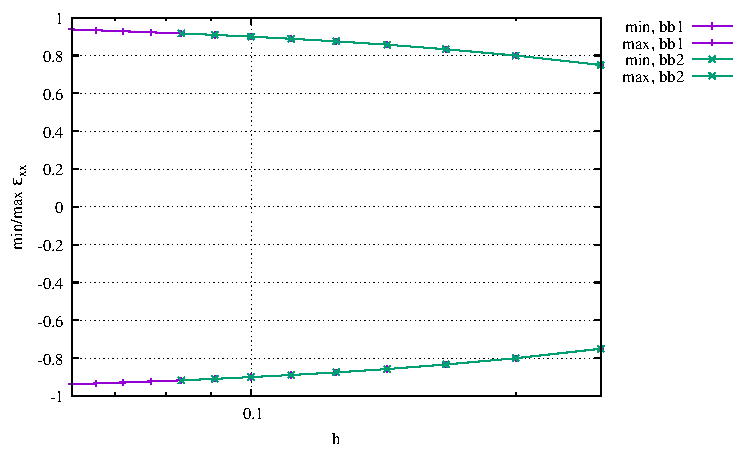
\includegraphics[width=5cm]{python_codes/fieldstone_75/results/mms3D/exx_stats.pdf}
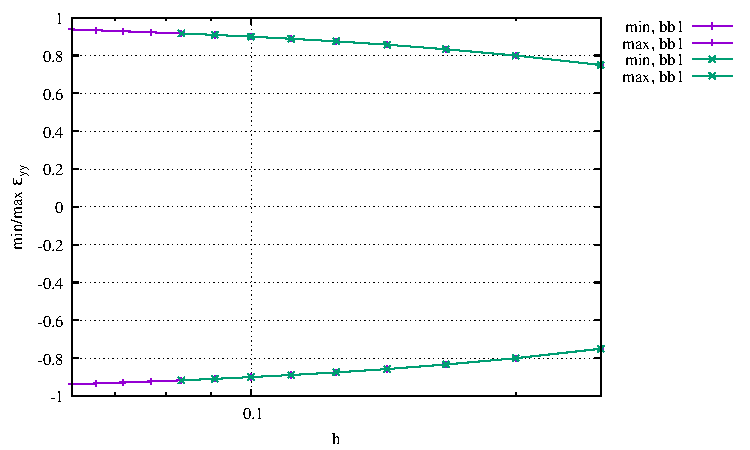
\includegraphics[width=5cm]{python_codes/fieldstone_75/results/mms3D/eyy_stats.pdf}
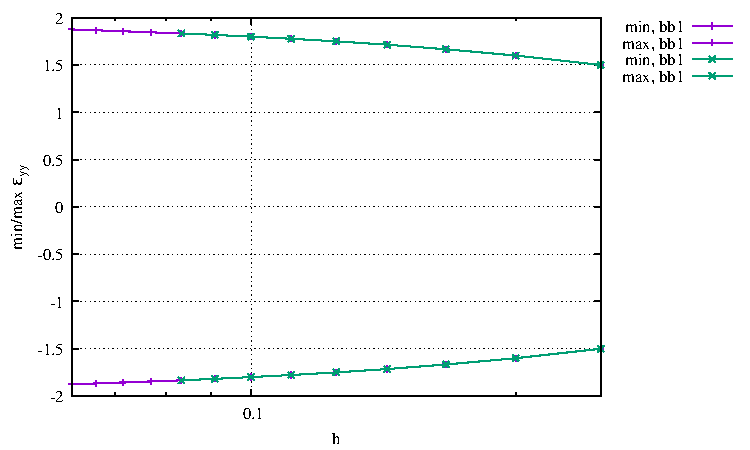
\includegraphics[width=5cm]{python_codes/fieldstone_75/results/mms3D/ezz_stats.pdf}\\
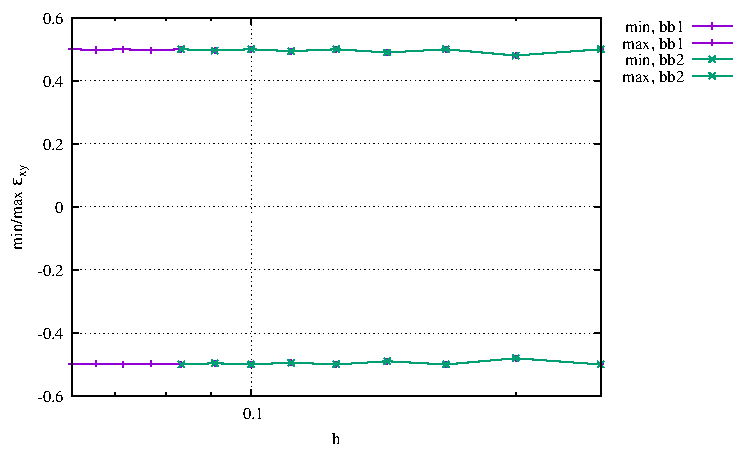
\includegraphics[width=5cm]{python_codes/fieldstone_75/results/mms3D/exy_stats.pdf}
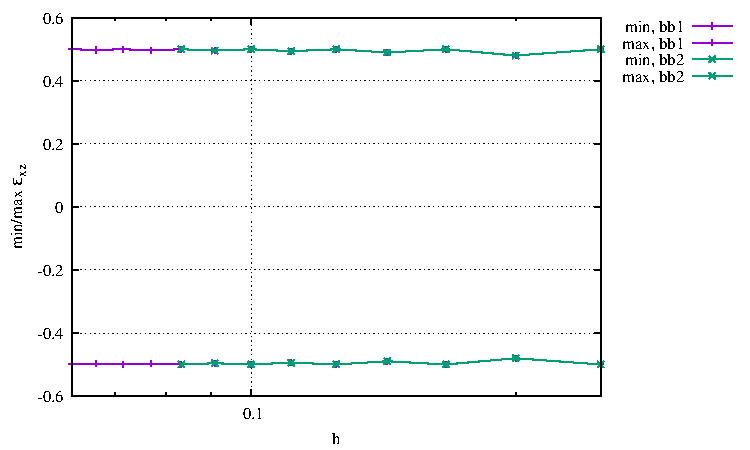
\includegraphics[width=5cm]{python_codes/fieldstone_75/results/mms3D/exz_stats.pdf}
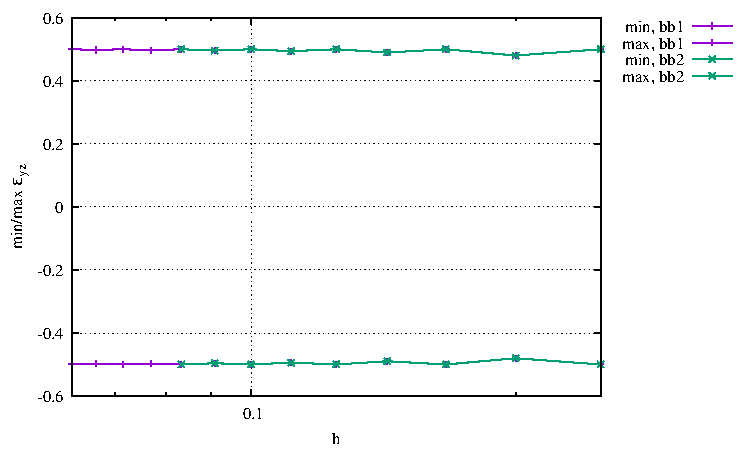
\includegraphics[width=5cm]{python_codes/fieldstone_75/results/mms3D/eyz_stats.pdf}\\
{\captionfont $\uparrow$ min/max statistics of the 6 components of the strain rate tensor
as a function of the mesh size $h$.}
\end{center}


\begin{center}
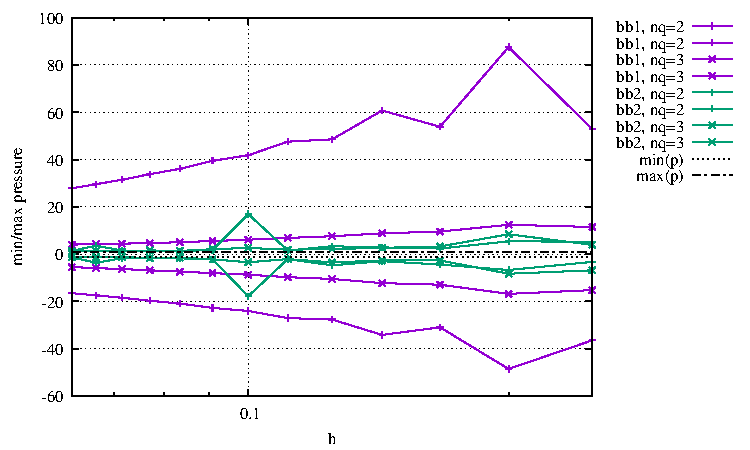
\includegraphics[width=11cm]{python_codes/fieldstone_75/results/mms3D/p_stats.pdf}\\
{\captionfont $\uparrow$ min/max statistics of the pressure as a function of the mesh size $h$.}
\end{center}


\begin{center}
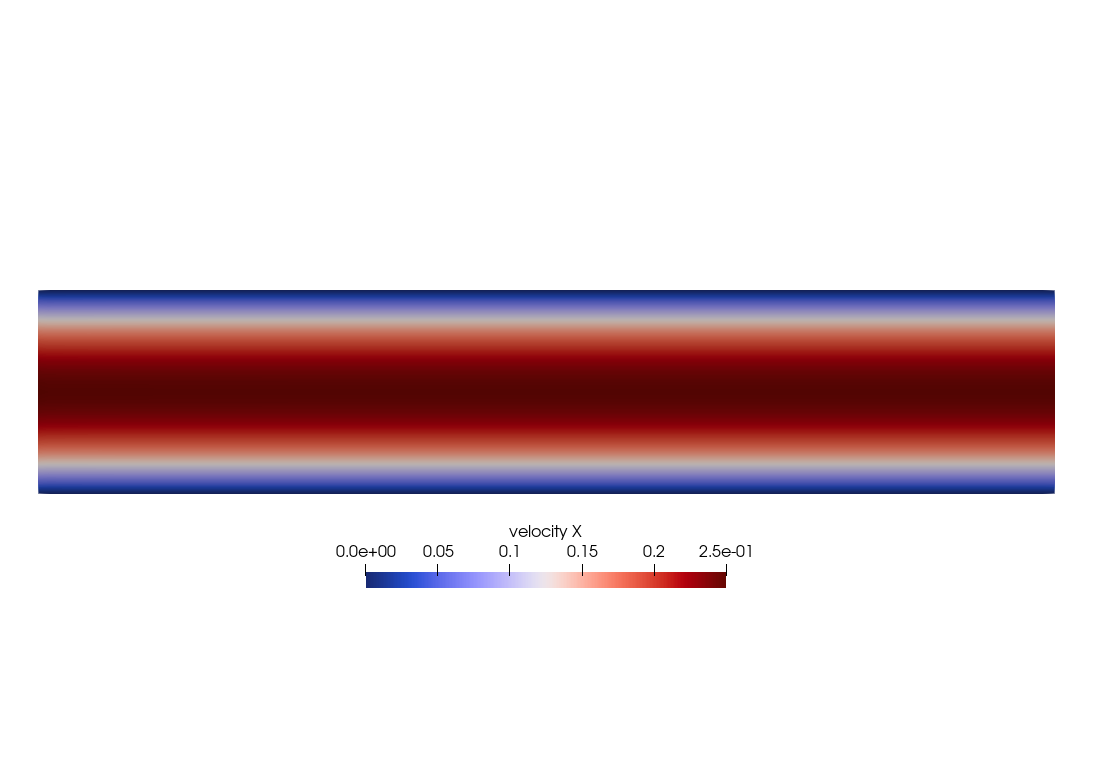
\includegraphics[width=5cm]{python_codes/fieldstone_75/results/mms3D/u}
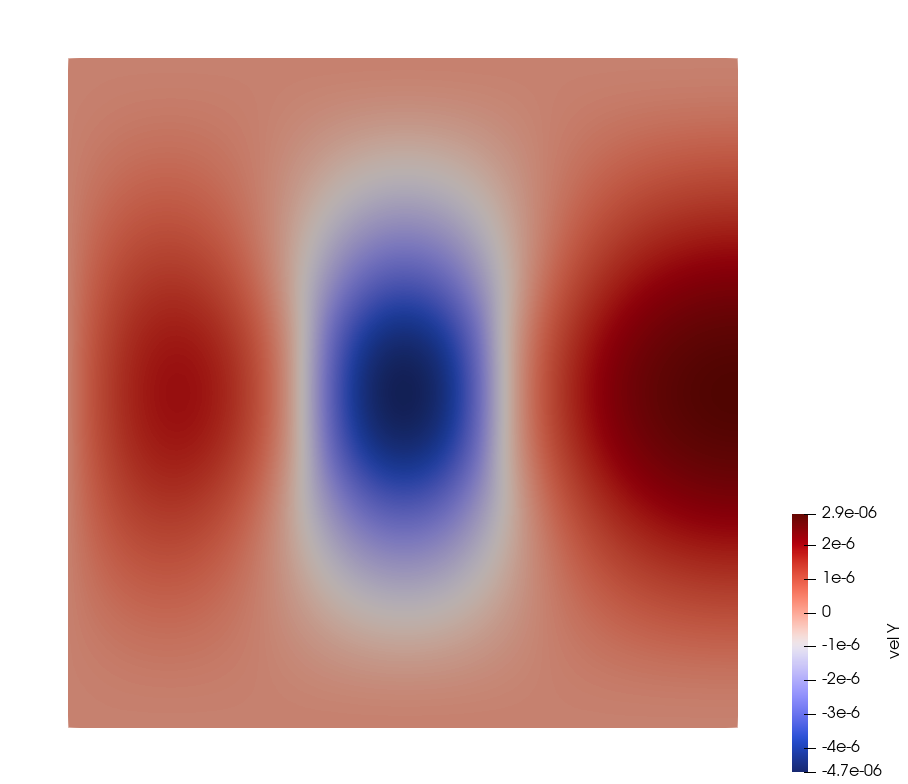
\includegraphics[width=5cm]{python_codes/fieldstone_75/results/mms3D/v}
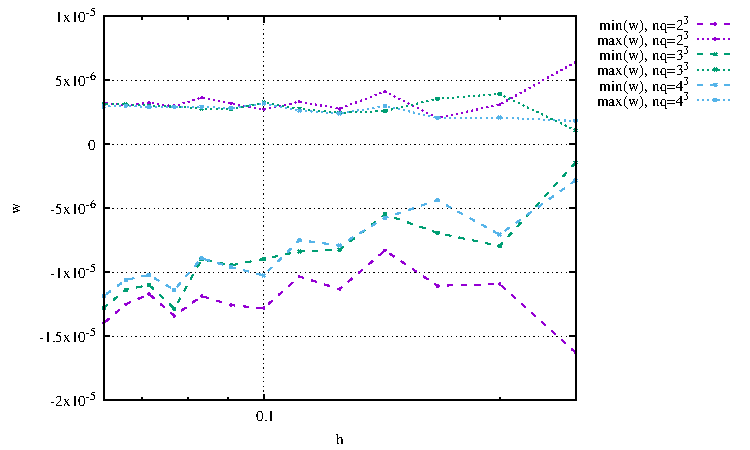
\includegraphics[width=5cm]{python_codes/fieldstone_75/results/mms3D/w}\\
\includegraphics[width=5cm]{python_codes/fieldstone_75/results/mms3D/vel}
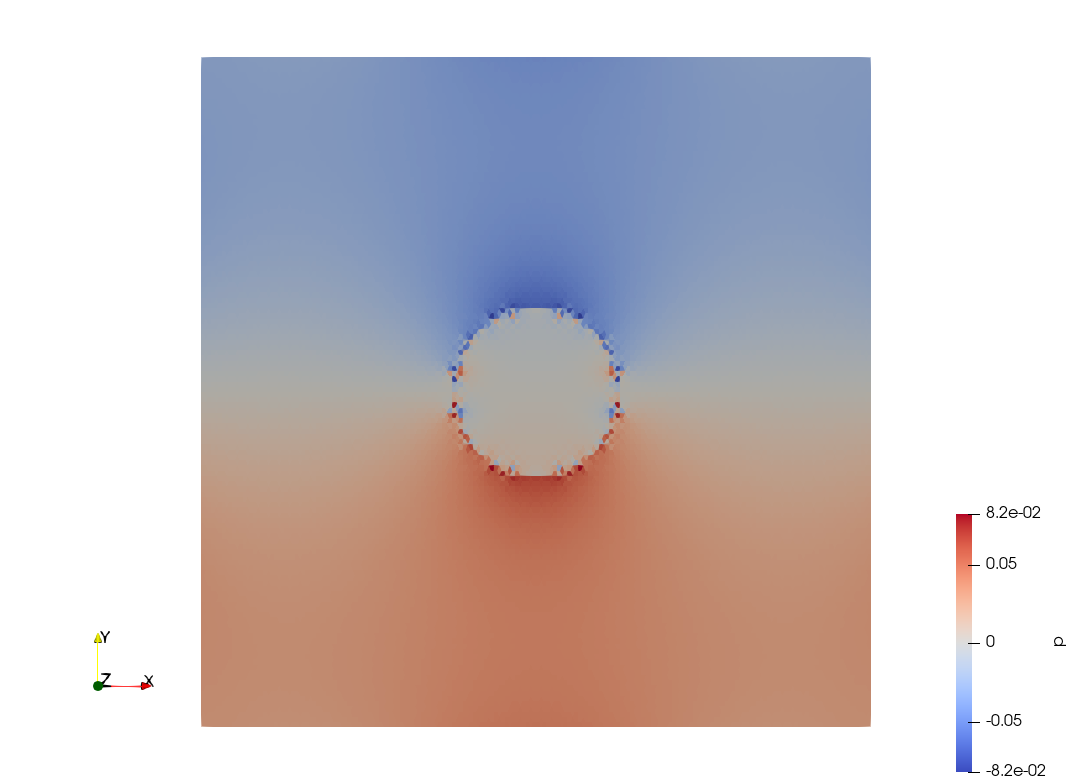
\includegraphics[width=5cm]{python_codes/fieldstone_75/results/mms3D/p}\\
{\captionfont $\uparrow$ Velocity and pressure fields (analytical fields)}
\end{center}

\begin{center}
\includegraphics[width=7cm]{python_codes/fieldstone_75/results/mms3D/p_b1}
\includegraphics[width=7cm]{python_codes/fieldstone_75/results/mms3D/p_b2}\\
{\captionfont Pressure field. Left: bubble \#1, Right: bubble \#2.}
\end{center}

Once again, the conclusion is clear: none of the two bubbles is capable of generating a 
smooth pressure field. Bubble 1 is objectively better than bubble 2.
It could be that my conclusions are limited by the lack of high resolution measurements
but the 2D experiments with the equivalent bubbles worked fine at low resolution...
